\documentclass[12pt,a4paper]{article}

\usepackage[in, plain]{fullpage}
\usepackage{array}
%\usepackage{../../../pas-math}
\usepackage{../../../moncours2}




\date{}
\title{\textcircled{{\normalsize{7}}} Fractions}

\graphicspath{{./img/}}


%\toggletrue{eleve}
%\toggletrue{dys}

%\rfoot{Page \thepage}
\begin{document}
	
	\maketitle



%\chap[num=3, color=red]{Fractions}{\today }

\begin{myobj}
	\begin{itemize}
		
		\item Construire le symétrique d’un point ou d'une figure par rapport à une droite à la main où à l’aide d’un logiciel;
		\item Construire le symétrique d’un point ou d'une figure par rapport à un point, à la main où à l’aide d’un logiciel;
		\item Utiliser les propriétés de la symétrie axiale ou centrale;
		\item Identifier des symétries dans des figures.		
	\end{itemize}
\end{myobj}

\begin{mycomp}
	\begin{itemize}
		\item \kw{Chercher (Ch2)} :  s’engager    dans    une    démarche    scientifique, observer, questionner, manipuler, expérimenter (sur une feuille de papier, avec des objets, à l’aide de logiciels), émettre des hypothèses, chercher des exemples ou des contre-exemples, simplifier ou particulariser une situation, émettre une conjecture ;
		\item \kw{Raisonner (Ra3)} :  démontrer : utiliser un raisonnement logique et des règles établies (propriétés, théorèmes, formules) pour parvenir à une conclusion ;
		\item \kw{Communiquer (Co2)} :  expliquer à l’oral ou à l’écrit (sa démarche, son raisonnement, un calcul, un protocole   de   construction   géométrique, un algorithme), comprendre les explications d’un autre et argumenter dans l’échange ; 
		
	\end{itemize}
\end{mycomp}




\section{Fraction et partage}


\begin{mydef}
	Lorsqu'on partage une unité en \kw{parts égales}, chaque part est une fraction de l'unité.
\end{mydef}

\begin{myex}
	
	La bande rouge ci-dessous représente l'unité.
	
	\begin{itemize}
		\item Elle est partagée en cinq parts de même dimensions.
		
		\begin{center}
			
\includegraphics[scale=0.42]{partage_1}
		\end{center}
	
		Chaque part représente un cinquième de la bande. On note $\dfrac{\textcolor{blue}{1}}{\textcolor{red}{5}}$.
		
		\item Si l'on colorie 3 parts, on colorie trois fois un cinquième, donc trois cinquièmes que l'on note $\dfrac{\textcolor{blue}{3}}{\textcolor{red}{5}}$. C'est une fraction.
		
		\begin{center}
			
			\begin{multicols}{2}
				
				\ \\
					
				
\includegraphics[scale=0.42]{partage_2}
				
				
				
				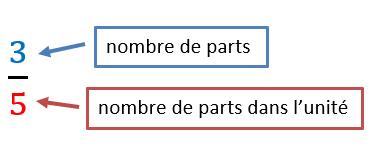
\includegraphics[scale=0.72]{exemple1}
			\end{multicols}
			
		\end{center}
	\end{itemize}
	
\end{myex}

\begin{mydef}
	Une fraction s'écrit sous la forme suivante :
	
	\begin{center}
		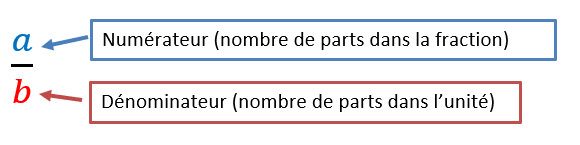
\includegraphics[scale=0.7]{definition}
	\end{center}
	
	où \textcolor{blue}{a} et \textcolor{red}{b} désignent deux nombres entiers, \textcolor{red}{b} est différent de zéro.
\end{mydef}

\section{Quotient et écriture fractionnaire}

	\begin{mydef}
		Le quotient des nombres $a$ et $b$ ($b$ $\neq$ 0), peut s'écrire sous la forme $\dfrac{a}{b}$.
	\end{mydef}

	\begin{myexs}
		\begin{itemize}
			\item  Le quotient $12 \div 36$ pur s'écrire sous la forme de la fraction $\dfrac{12}{36}$.
			
			\item L'écriture fractionnaire $\dfrac{\num{8,2}}{2}$ correspond au quotient $\num{8,2} \div 2$
		\end{itemize}
	\end{myexs}

	\begin{myprops}
		
		\begin{itemize}
			\item Une fraction où le numérateur est inférieur au dénominateur est inférieure à 1. 
			\item Une fraction où le numérateur est supérieure au dénominateur est supérieure à 1.
		\end{itemize}
	\end{myprops}

	\begin{myexs}
		\begin{itemize}
			\item  $\dfrac{3}{4} < 1$ ($3 \div 4 = \num{0.75}$).
			
			\item $\dfrac{23}{5} > 1$ ($23 \div 5 = \num{4.6}$).
		\end{itemize}
	\end{myexs}

\newpage

\section{Fractions et repérages}

\subsection{Placer une fraction sur une demi-droite graduée}


\begin{mymeth}
	
	\iftoggle{eleve}{%
		Pour \hrulefill %\\
		
		\vspace*{0.2cm}
		\hrulefill
		
		\vspace*{0.2cm}
		\hrulefill
	}{%
		Pour repérer la fraction $\dfrac{\textcolor{blue}{a}}{\textcolor{red}{b}}$, on partage l'unité en \textcolor{red}{b} segments de même longueur, puis in reporte \textcolor{blue}{a} fois cette longueur à partir de zéro.
	}
	
\end{mymeth}

\begin{myex}
	
	\iftoggle{eleve}{%
		On \hrulefill
		
		\begin{itemize}
			\item on \hrulefill
			\item on \hrulefill
		\end{itemize}
	}{%
		On veut repérer la fraction
		
		$\dfrac{\textcolor{blue}{8}}{\textcolor{red}{5}}$ :
		
		\begin{itemize}
			\item on partage l'unité en \textcolor{red}{5} segments de même longueur
			\item on reporte \textcolor{blue}{8} fois cette longueur.
		\end{itemize}
	}
	
	
	
\end{myex}

\subsection{Encadrer une fraction}

\begin{myprop}
	
	\iftoggle{eleve}{%
		On \hrulefill
		
		\vspace*{0.2cm}
		\hrulefill
		
		
		\vspace*{0.2cm}
		\hrulefill
		
		\begin{equation*}
			 \leq \dfrac{a}{b} < 
		\end{equation*}
		
		Où \hrulefill 
		
		\vspace*{0.2cm}
		\hrulefill
	}{%
		On peut encadrer n'importe quelle fraction par deux nombres entiers consécutifs . %(qui se suivent).
		
		Si $a$ et $b$ sont deux nombres entiers ($b \neq 0$), on a :
		
		\begin{equation*}
			\textcolor{red}{q} \leq \dfrac{a}{b} < \textcolor{red}{q}+1
		\end{equation*}
		
		Où \textcolor{red}{q} est le quotient de la division euclidienne de $a$ par $b$.
	}
	
\end{myprop}

\begin{myex}
	On veut encadrer $\dfrac{123}{17}$ par deux nombres entiers consécutifs. \\
	
	
	\iftoggle{eleve}{%
		\vspace*{0.2cm}
		\hrulefill
		
		
	}{%
		On a $123 = 17 \times \textcolor{red}{7} + 4$. Donc 
		
		\begin{equation*}
			\textcolor{red}{7} \leq \dfrac{123}{17} < 8.
		\end{equation*}
	}
	
	
\end{myex}


\newpage

\section{Fraction d'une quantité}

\begin{myprop}
	
	\iftoggle{eleve}{%
		Pour \hrulefill 
		
		\vspace*{0.2cm}
		\hrulefill 
	}{%
		Pour prendre une fraction d'une quantité on multiplie cette quantité par la fraction.
	}
	
\end{myprop}

\begin{myex}
	Combien font $\dfrac{3}{4}$ de 20 € ?
	
	
	\iftoggle{eleve}{%
		
		\vspace*{0.2cm}
		\hrulefill 
		
		\vspace*{0.4cm}
		\hrulefill 
	}{%
		\begin{equation*}
			20 \times \dfrac{3}{4} = 20 \times 3 \div 4 = 20 \times \num{0.75} = 15
		\end{equation*}
	
		Les trois quarts de 20 € font 15 €
	}
	

	
\end{myex}

\vspace*{-0.2cm}

\section{Comparaison de fractions}

\iftoggle{eleve}{%
	\begin{myprop}
		Deux \hrulefill
		
		\vspace*{0.2cm}
		\hrulefill
	\end{myprop}
	
	\begin{myex}
		On \hrulefill
		
		\vspace*{0.4cm}
		\hrulefill
	\end{myex}
	
}{%
	\begin{myprop}
		Deux fractions avec le même dénominateur sont rangées dans le \kw{même ordre que leur numérateurs}.
	\end{myprop}
	
	\begin{myex}
		On veut comparer $\dfrac{3}{4}$ et $\dfrac{1}{4}$ :
		
		$3 > 1$ donc $\dfrac{3}{4} > \dfrac{1}{4}$.
	\end{myex}
	
}


\section{Autres écritures d'une fraction}

\subsection{Fractions égales}

\begin{myprop}
	
	\iftoggle{eleve}{%
		Un \hrulefill 
		
		\vspace*{0.2cm}
		\hrulefill 
		
		\vspace*{0.2cm}
		\hrulefill 
	}{%
		Un quotient ne change pas quand on multiplie (ou divise) son numérateur et son dénominateur par un même nombre non nul.
	}
	
\end{myprop}


\begin{myexs}
	\begin{itemize}
		\iftoggle{eleve}{%
			\item \vspace*{0.2cm}
			\hrulefill
			
			\item \vspace*{0.2cm}
			\hrulefill
		}{%
			\item $\dfrac{1}{2} = \dfrac{1 \times 2}{2 \times 2} = \dfrac{2}{4}$ 
			\item $\dfrac{2}{6} = \dfrac{2 \div 2}{6 \div 2} = \dfrac{1}{3}$ , ici on  a simplifié par 2, la fraction $\dfrac{2}{6}$.
		}
	\end{itemize}
\end{myexs}

\subsection{Fractions décimales}

\iftoggle{eleve}{%
	\begin{mydef}
		Une
		\hrulefill 
		
		\vspace*{0.2cm}
		\hrulefill 
	\end{mydef}
	
	\begin{myprop}
		Tout
		\hrulefill 
		
		\vspace*{0.2cm}
		\hrulefill 
	\end{myprop}
	
	\begin{myexs}
		\begin{multicols}{2}
			\begin{itemize}
				\item \ %$\dfrac{25}{10} = \num{2.5}$
				\item \ %$\dfrac{25}{1000} = \num{0.025}$
				\item \ %$\num{32.54} = \dfrac{3254}{100}$
				\item \ %$\num{0.2} = \dfrac{2}{10}$
				
			\end{itemize}
		\end{multicols}
	\end{myexs}
}{%
	\begin{mydef}
		Une fraction décimale est une fraction dont le dénominateur est un multiple de 10.
	\end{mydef}
	
	\begin{myprop}
		Tout nombre décimal peut s'écrire sous forme de fraction décimale
	\end{myprop}
	
	\begin{myexs}
		\begin{multicols}{2}
			\begin{itemize}
				\item $\dfrac{25}{10} = \num{2.5}$
				\item $\dfrac{25}{1000} = \num{0.025}$
				\item $\num{32.54} = \dfrac{3254}{100}$
				\item $\num{0.2} = \dfrac{2}{10}$
				
			\end{itemize}
		\end{multicols}
	\end{myexs}
}


%
%\begin{mydef}
	$a$ et $b$ sont deux nombres ($b$ $\neq$ 0). Le \hspace{3cm} de $a$ par $b$ se note $a \div b$ ou $\dfrac{a}{b}$, en \hspace{5cm}.
\end{mydef}

\begin{myex}
	%\begin{itemize}
		%\item 
		Le quotient de 5 par 4 est $\dfrac{5}{4}$, c'est le nombre qui multiplié par 4 donne 5. 
		\begin{equation*}
			\dfrac{5}{4} \times 4 = 
		\end{equation*}

		%\item Le quotient de 2 par 3 est $\dfrac{2}{3}$, c'est le nombre qui multiplié par 3 donne 2. $\dfrac{2}{3} \times 3 = 2 $.
	%\end{itemize}
\end{myex}

\begin{mydef}
	Si $a$ et $b$ sont entiers, alors $\dfrac{a}{b}$ est une \hspace{3cm}. $a$ est le \hspace*{3cm} et $b$ est le \hspace*{3cm}.	
	
\end{mydef}

\begin{center}
	\includegraphics*[scale=0.5]{def_2}
\end{center}

\begin{myex}
	$\dfrac{\num{4.2}}{\num{2}}$, $\dfrac{\num{5}}{\num{2.4}}$, $\dfrac{\num{1.3}}{\num{3.7}}$ et $\dfrac{\num{2}}{\num{3}}$ sont toutes des écritures fractionnaires, mais seule \hspace{2cm} est une fraction.
\end{myex}
%
%\newpage
%\section{Divisibilité et nombres premiers}
%
%\begin{myprop}
	Un nombre $a$ est \hspace*{3cm}par un nombre $b$ si le reste de la division de $a$ par $b$ vaut 0. 
\end{myprop}

\begin{myexs}
	\begin{itemize}
		\item $ 5 \times 3 + 0 = 15$, donc 15 \hspace*{5cm}.
		\item $ 5 \times 3 + 2 = 17$, donc 17 \hspace*{5cm}.
	\end{itemize}
\end{myexs}

\begin{myprops}
	\begin{itemize}
		\item Un nombre est divisible par 2 s'il est \hspace*{2cm} (son chiffre des unités est 0, 2, 4, 6 ou 8).
		\item Un nombre est divisible par 3 si la \hspace*{6cm} est divisible par 3.
		\item Un nombre est divisible par 5 si son chiffre des unités est \hspace*{2cm}.
		\item Un nombre est divisible par 9 si la somme de ses chiffres est \hspace*{3cm}. 
	\end{itemize}
\end{myprops}

\begin{myexs}
	\begin{itemize}
		\item 20 est divisible par %2 et 5;
		\item 45 est divisible par %3, 5 et 9 (4 + 5 = 9);
		\item 2520 est divisible par %2, 3, 5 et 9 (2 + 5 + 2 =9 ).
	\end{itemize}
\end{myexs}

\begin{myprops}
	\begin{itemize}
		\item Un \hspace*{5cm} est un nombre qui est divisible uniquement par 1 et lui-même.	
		
		\item Les nombres premiers inférieurs à 30 sont : 1; 2; 3; 5; 7; 11; 13; 17; 19; 23 et 29. 
	\end{itemize}
	
\end{myprops}

\begin{myexs}
	\begin{itemize}
		\item 15 est divisible par 3 et 5, il n'est pas premier.
		\item 21 est divisible par 3 et 7, il n'est pas premier.
	\end{itemize}
\end{myexs}
%
%\section{Fractions égales et simplification}

%\setcounter{section}{3}

%\section{\'Egalité des produits en croix}

%\begin{myprop}
	$a$, $b$, $c$ et $d$  sont des nombres entiers avec \\
	
	$\dfrac{a}{b} = \dfrac{c}{d}$ signifie que  
	
	 
\end{myprop}


\begin{myexs}
	\begin{itemize}
		\item $\dfrac{34}{51} = \dfrac{2}{3}$ car $34 \times 3 = 51 \times 2 = 102$
		
		\item Je veux compléter $\dfrac{23}{15} = \dfrac{207}{?}$
		
		On a :
		
		\begin{eqnarray*}
			23 \times ... &=&  \\
			23 \times ... &=&  \\
		\end{eqnarray*}
		
		Je calcule $\num{3105} \div 23 =  $ \\
		
		Donc $\dfrac{23}{15} = $
	\end{itemize}
	
\end{myexs}


\end{document}